%\documentclass[12pt,a4paper,twoside]{book} 
\usepackage[spanish]{babel} % de pedro
\usepackage{graphics,graphicx,epsfig,color,float,afterpage,fancyheadings,subfigure,moreverb,alltt} % de pedro
\usepackage[latin1]{inputenc} % tildes de pedro

\usepackage{algorithm}
\usepackage{algorithmic}

\usepackage{rotating}
\usepackage{url}

%% Esta letra se convierte mejor a pdf que la normal
\usepackage{ae}

%%% Para las fuentes matemticas
\usepackage{amsfonts}

\usepackage{subfigure}

\usepackage{pstricks} % para los dibujos del da
\usepackage{lscape} % para las pginas en horizontal
\usepackage{portland} % para las pginas en horizontal
\usepackage{supertabular} % para las tablas de ms de una pgina
\usepackage{tabularx} % para las tablas del tipo tabularx
%\usepackage{glossary}
%\documentclass[a4paper,spanish,12pt]{book} % esto es de gustavo
%\usepackage{amsmath,amsfonts}   % underset mathbb
%\usepackage{authordate1-4}      % bib style
%\usepackage{epsfig}     % eps
\usepackage{epic}           % graficos
%\usepackage{eepic}           % graficos
\usepackage{curvesls}           % curvas
\usepackage{amssymb}
%\usepackage{fancyheadings}  % encabezados
%\usepackage{hhline}             % hhline
%\usepackage[latin1]{inputenc}   % tildes
%\usepackage{makeidx}        % ndices
%\usepackage{setspace}           % interlinea
%\usepackage[spanish]{babel} % espaol

%%%%%%%%%%%%%%%%%%%%%%%%%%%%%%%%%%%%%%%%%%%%%%%%%%%%%%%%%%%%%%%%%%%%%%%%%%%%%%%

\author{juanlu}
\title{Tesis de Juan Lus Jimnez Laredo}




\newcommand{\fecha}{\footnotesize{[ Impreso: \the\day-\ifcase\month\or
    Ene\or Feb\or Mar\or Abr\or May\or Jun\or Jul\or Ago\or Sep\or
      Oct\or Nov\or Dic\fi-\the\year ]}}

\newcommand{\N}{\mathbb{N}}

%% Para corregir las cabeceras largas
\newcommand{\cabecera}[2]{
\markright{\ref{#1}. \hspace{0.1ex} \MakeUppercase{#2}}}


%\pagestyle{headings}
%\renewcommand{\chaptermark}[1]{\markboth{\fecha \\ \\ #1}{}}
%\renewcommand{\sectionmark}[1]{\markright{#1 \\ \\ \fecha}}
%\addtolength{\headheight}{2.5pt}



%\lhead[\it\thechapter]{\sl\rightmark}
%\rhead[\rm\leftmark]{\it\thesection}
%\rfoot[]{\thepage}
%\cfoot[]{}
%\lfoot[\thepage]{}

%\thispagestyle{plain}

\setcounter{secnumdepth}{3}
\setcounter{tocdepth}{3}

%\renewcommand{\baselinestretch}{1.2}
%\setlength{\parskip}{0.8ex}

\newtheorem{theorem}{\sf Teorema}
\newtheorem{lemma}{\sf Lema}

\newcommand{\rem}[1]{\S\iffalse #1 \fi}
\newcommand{\cur}[1]{ {\it #1\/} }
\newcommand{\crcl}[1]{#1\kern-9pt\raise1pt\hbox{$\bigcirc$}}
\newcommand{\evag}{{\sf EvAg}}
\newcommand{\evagp}{{\sf EvAg.}}
\newcommand{\evags}{{\sf EvAgs}}
\newcommand{\evagsp}{{\sf EvAgs.}}

\newcommand{\prog}[2] {
   \small
   \begin{minipage}[t]{75mm} {\tt #1}  \end{minipage}
   \begin{minipage}[t]{60mm} {#2}      \end{minipage}
   \\
}
\newcommand{\prg}[2] { {\tt #1} & {\sf #2} \\}

\newcommand{\wmfspecial}[4]{
   \begin{figure}[h]
   \centerline{\psfig{figure=#1,height=#2}}
   \caption{#3}   \label{#4}
   \end{figure}
}                   % USO: \wmfspecial{nombre.eps}{altura}{leyenda}{etiqueta}

\def\stackunder#1#2{\mathrel{\mathop{#2}\limits_{#1}}}

\def\marco #1#2#3#4{\centerline{       % USO: \marco{.1}{10}{124mm}
  \vbox{\hrule height #1pt%
  \hbox{\vrule width #1pt\kern #2pt%
  \vbox{\kern #2pt%
  \vbox{\hsize #3\noindent #4}%
  \kern #2pt}%
  \kern #2pt\vrule width #1pt}%
  \hrule height0pt depth #1pt}} }


\newcommand{\symnote}[2]{\symbolnote{#1}{#2}}

\newfont{\bi}{cmbxti10 scaled\magstep1}       % bf + it


%% Ruta de las figuras
\graphicspath{{../figuras/}}


\begin{document}
           % Eliminarlo al compilar el documento maestro, ponerlo para compilarlo separado

%%%%%%%%%%%%%%%%%%%%%%%%%%%%%%%%%%%%%%%%%%%%%%%%%%%%%%%%%%%%%%%%%%%%%%%%%%%%%%%
%%                                                                           %%
%%                             Tesis Doctoral:                               %%
%%                        Juan Luis Jimenez Laredo                           %%
%%                                                                           %%
%%%%%%%%%%%%%%%%%%%%%%%%%%%%%%%%%%%%%%%%%%%%%%%%%%%%%%%%%%%%%%%%%%%%%%%%%%%%%%%

\cabecera{cap:p2pcompt}{Peer-to-Peer Computing} %Descomentarlo para compilar maestro
\chapter{\textit{Newscast in the context of Peer-to-Peer Computing}}
\label{cap:p2pcompt}
\cabecera{cap:p2pcompt}{Peer-to-Peer Computing} %Descomentarlo para compilar maestro

%%%%%%%%%%%%%%%%%%%%%%%%%%%%%%%%%%%%%%%%%%%%%%%%%%%%%%%%%%%%%%%%%%%%%%%%%%%%%%%

%Peer-to-Peer computing is the general term describing all issues related
%to P2P systems.  % Menuda tautología! - JJ
%Such issues include protocols development, security
%management, analysis of performance or application areas
%\cite{DBLP:conf/p2p/2005lncs}.

By the term Peer-to-Peer computing we will refer to those issues relating to protocol development, security management, analysis of performance and applications of P2P systems \cite{DBLP:conf/p2p/2005lncs}. 
% Una tautología menos tautológica - Juanlu

Peers (that will be also referred to as \emph{nodes} in the context of
communication graphs) are equal entities able to establish a
self-organised and decentralised communication using their own routing
mechanisms. Therefore, the working principle of the P2P technology
is the ability of every \emph{peer} to behave autonomously as a
\emph{servent}, that is, every peer acts as a SERVer and a
cliENT.

Such a dual operational mode has been proved to be a good way to
harness decentralised resources at the \emph{edges} of the network
(e.g. storage or computing power), giving a single coherent view of the
system. Taking adventage of such features, the aim of this thesis is using P2P technology as a computing platform in the application area of Evolutionary Algorithms. 

In order to explain the design decisions taken further on the following chapters and put EAs in the context of P2P technology, Section \ref{sec:p2ptaxonomy} reviews different taxonomies of P2P systems according to criteria such as system architectures or application areas. In such a framework, Section
\ref{sec:p2pnewscast} analyses the specific protocol that will be used throughout this thesis, the \emph{newscast}
protocol. It consists in a fully-decentralised protocol firstly proposed in \cite{jelasity:newscast} by Jelasity and van Steen which has shown to succeed in the main issues related to P2P computing such as massive scalability or fault tolerance in e.g. \cite{jelasity:gossip,spyros:robustscalable,peersampling}. 
%dives in es muy inespecífico. Di que consigue con éxito afrontar todos
%los problemas que plantean los sistemas P2P - JJ
%Cambios introducidos - Juanlu
 Finally, Section \ref{sec:p2pconclusions} concludes with a summary about the described technologies stating how an easy understandable protocol such as newscast is representative of the P2P paradigm.
%Deja siempre bien claro lo que estás haciendo para esta tesis y lo que
%no. - JJ
%Modificada la referencia a la última sección. - Juanlu
 

\section{Taxonomies of P2P systems}
\label{sec:p2ptaxonomy}
%%%%%%%%%%%%%%%%%%%%%%%%%%%%%%%%%%%%%%%%%%%%%%%%%%%%%%%%%%%%%%%%%%%%%%%%%%%%%%%

In order to present the main issues involving P2P systems and how different applications approaches take adventage of P2P technology, this section explains two well-known methods for classifying P2P systems; the first one, in Section \ref{sec:p2parchitecture}, classifies P2P systems according to the degree of decentralisation promoted by different kind of system architectures, meanwhile, the second one, in Section \ref{sec:p2papplication}, provides a taxonomy on the different application areas of P2P systems.


\subsection{System architecture}
\label{sec:p2parchitecture}
%%%%%%%%%%%%%%%%%%%%%%%%%%%%%%%%%%%%%%%%%%%%%%%%%%%%%%%%%%%%%%%%%%%%%%%%%%%%%%%

The harnessing of resources in P2P systems depends of three basic features of the architecture design, resource availability, resource discovery and resource retrieval. Availability and retrieval of resources refer to the way in which resources are disposed within the system, and therefore, the way in which they can be retrieved. Additionally, the discovery of resources addresses the {\em look-up} of contents in large and decentralised systems.


In Bittorrent \cite{bittorrent:understanding}, for example, files are available in pieces of equal size in a distributed network known as swarm. Two kind of special peers, seeders and trackers, have respective information on the location of pieces and peers. This way, seeders and trackers allow a client to discover the resources, so that, it can retrieve content from the swarm in a decentralised fashion. 
%Despite being a very efficient protocol, a major drawback of Bittorrent was trackers representing a critical point for the discovery of resources. A tracker failure prevented the {\em look-up} of content.

Nevertheless, an efficient {\em look-up} mechanism turns out to be not trivial for large and decentralised systems. In this sense, the system architecture mainly depends on decisions about the indexing and discovery of resources and according to such design decisions, P2P architectures can be classified within the following three main blocks:


\subsubsection{Centralised}

    The \emph{look-up} service is implemented on central servers, and therefore, all the addressable content of the peers is centralised such as in Napster \cite{napstervsgnutella}. The major drawback of centralised systems is that servers represent a possible bottleneck for massive scalability and a single point of failure. A good example is the history of Napster itself. Its controversial use for the illegal sharing of copyright protected files in addition with its centralised look-up architecture led soon to the intervention of the service in 2001 by simply closing the servers. 

\subsubsection{Decentralised}
    
    In order to cope with the limitations of centralised approaches, decentralised alternatives such as Gnutella 0.4 \cite{gnutella04} have emerged during the last decade. In a nutshell, a decentralised system implies that many nodes are providers of the \emph{look-up} service making the system robust to failures of punctual nodes.

    Such kind of approach has shown to be massively scalable and is imposing within the current P2P architectures. The great number of P2P systems following a decentralised scheme requires of an additional subclassification. The most extended criterion for it is considering whether the peers do a pro-active effort to maintain a given network topology (in this case they are known as structured systems) or the properties of the network emerge from the collective behaviour of the peers (known as unstructured systems).

\begin{itemize}
\item {\bf Structured systems}: 

    It mainly refers to distributed hash table approaches (DHT) such as Chord \cite{chord}, Pastry \cite{pastry}, Tapestry \cite{tapestry} or CAN \cite{can}. DHTs consist in the distributed indexing of contents using pairs $(key,value)$. To this aim, the key space is composed of a set of integer values, e.g. from 0 to $2^{80}$. Any node within the network receives a portion of key indexes and a routing table to $l$ different nodes in such a way that entries point to nodes at the position $n+2^{i-1}$, where $1 \le i \le l$ and $n$ is the current node. This way, the \emph{look-up} of a given $key$ can be done in $O(log(n))$ steps.


\item {\bf Unstructured systems}: 

    Some authors also refer to such systems as Pure P2P \cite{DBLP:conf/p2p/2005lncs}. The main idea behind is that all elements in the system are distributed without any central component. Examples of these systems are Gnutella 0.4 \cite{gnutella04} or newscast \cite{jelasity:newscast}. Decisions on the routing are taken locally by every peer, and therefore, the network topology is self-organised. In these systems, the \emph{look-up} for contents is based on flooding mechanisms (a.k.a. gossipping or epidemic \emph{look-up}), that is, a request is flooded through neighbour nodes taking a certain number of hops. The key to success is the small diameter of the network at the self-organised small-world relationship between nodes. Hence, a given \emph{look-up} could take $log(n)$ hops with respect to a network of size $n$.
\end{itemize}

\subsubsection{Hybrid or semi-centralised}

    Finally, there are hybrid (or semi-centralised) approaches consisting in a hub based architecture. Hubs, also known as Superpeers, have a higher degree of connections than the rest of peers, known as leafnodes. Despite hubs representing a sort of centralisation, they scale according to the network size. That is, the architecture allows massive scalability by increasing the number of superpeers with respect to the network size. On the other hand, the degree of leafnodes also scales following a power-law distribution. A good example of hybrid architecture is Gnutella 0.6 \cite{gnutella06} whose aim was to reduce the load of the network with respect to the decentralised version, Gnutella 0.4.


\subsubsection{Summary}

As a summary, Figure \ref{fig:p2parchitectures} depicts the topologies of the three system architectures. In order to study the viability of P2P EAs, we have chosen newscast (a purely decentralised P2P system \cite{jelasity:newscast}) as the system architecture for this thesis. As it will be analysed in Section \ref{sec:p2pnewscast}, newscast adopts the shape of a complex network and fits with all the requirements exposed in the previous Chapter for a fine-grained P2P EA such as decentralisation, massive-scalability or fault tolerance. In this sense, choosing a centralised approach would have imposed some limitations on the scalability in addition to the high vulnerability to failures on central nodes. On the other hand, hybrid approaches are the response that arise from issues related to load balancing the network traffic or the computing power. We find that such issues would correspond to decisions in later phases of design rather than in a preliminary study of viability.


\begin{figure}[htbp]
\centering
\subfigure{\includegraphics[width=0.4\textwidth]{clienteservidor}}\\
\subfigure{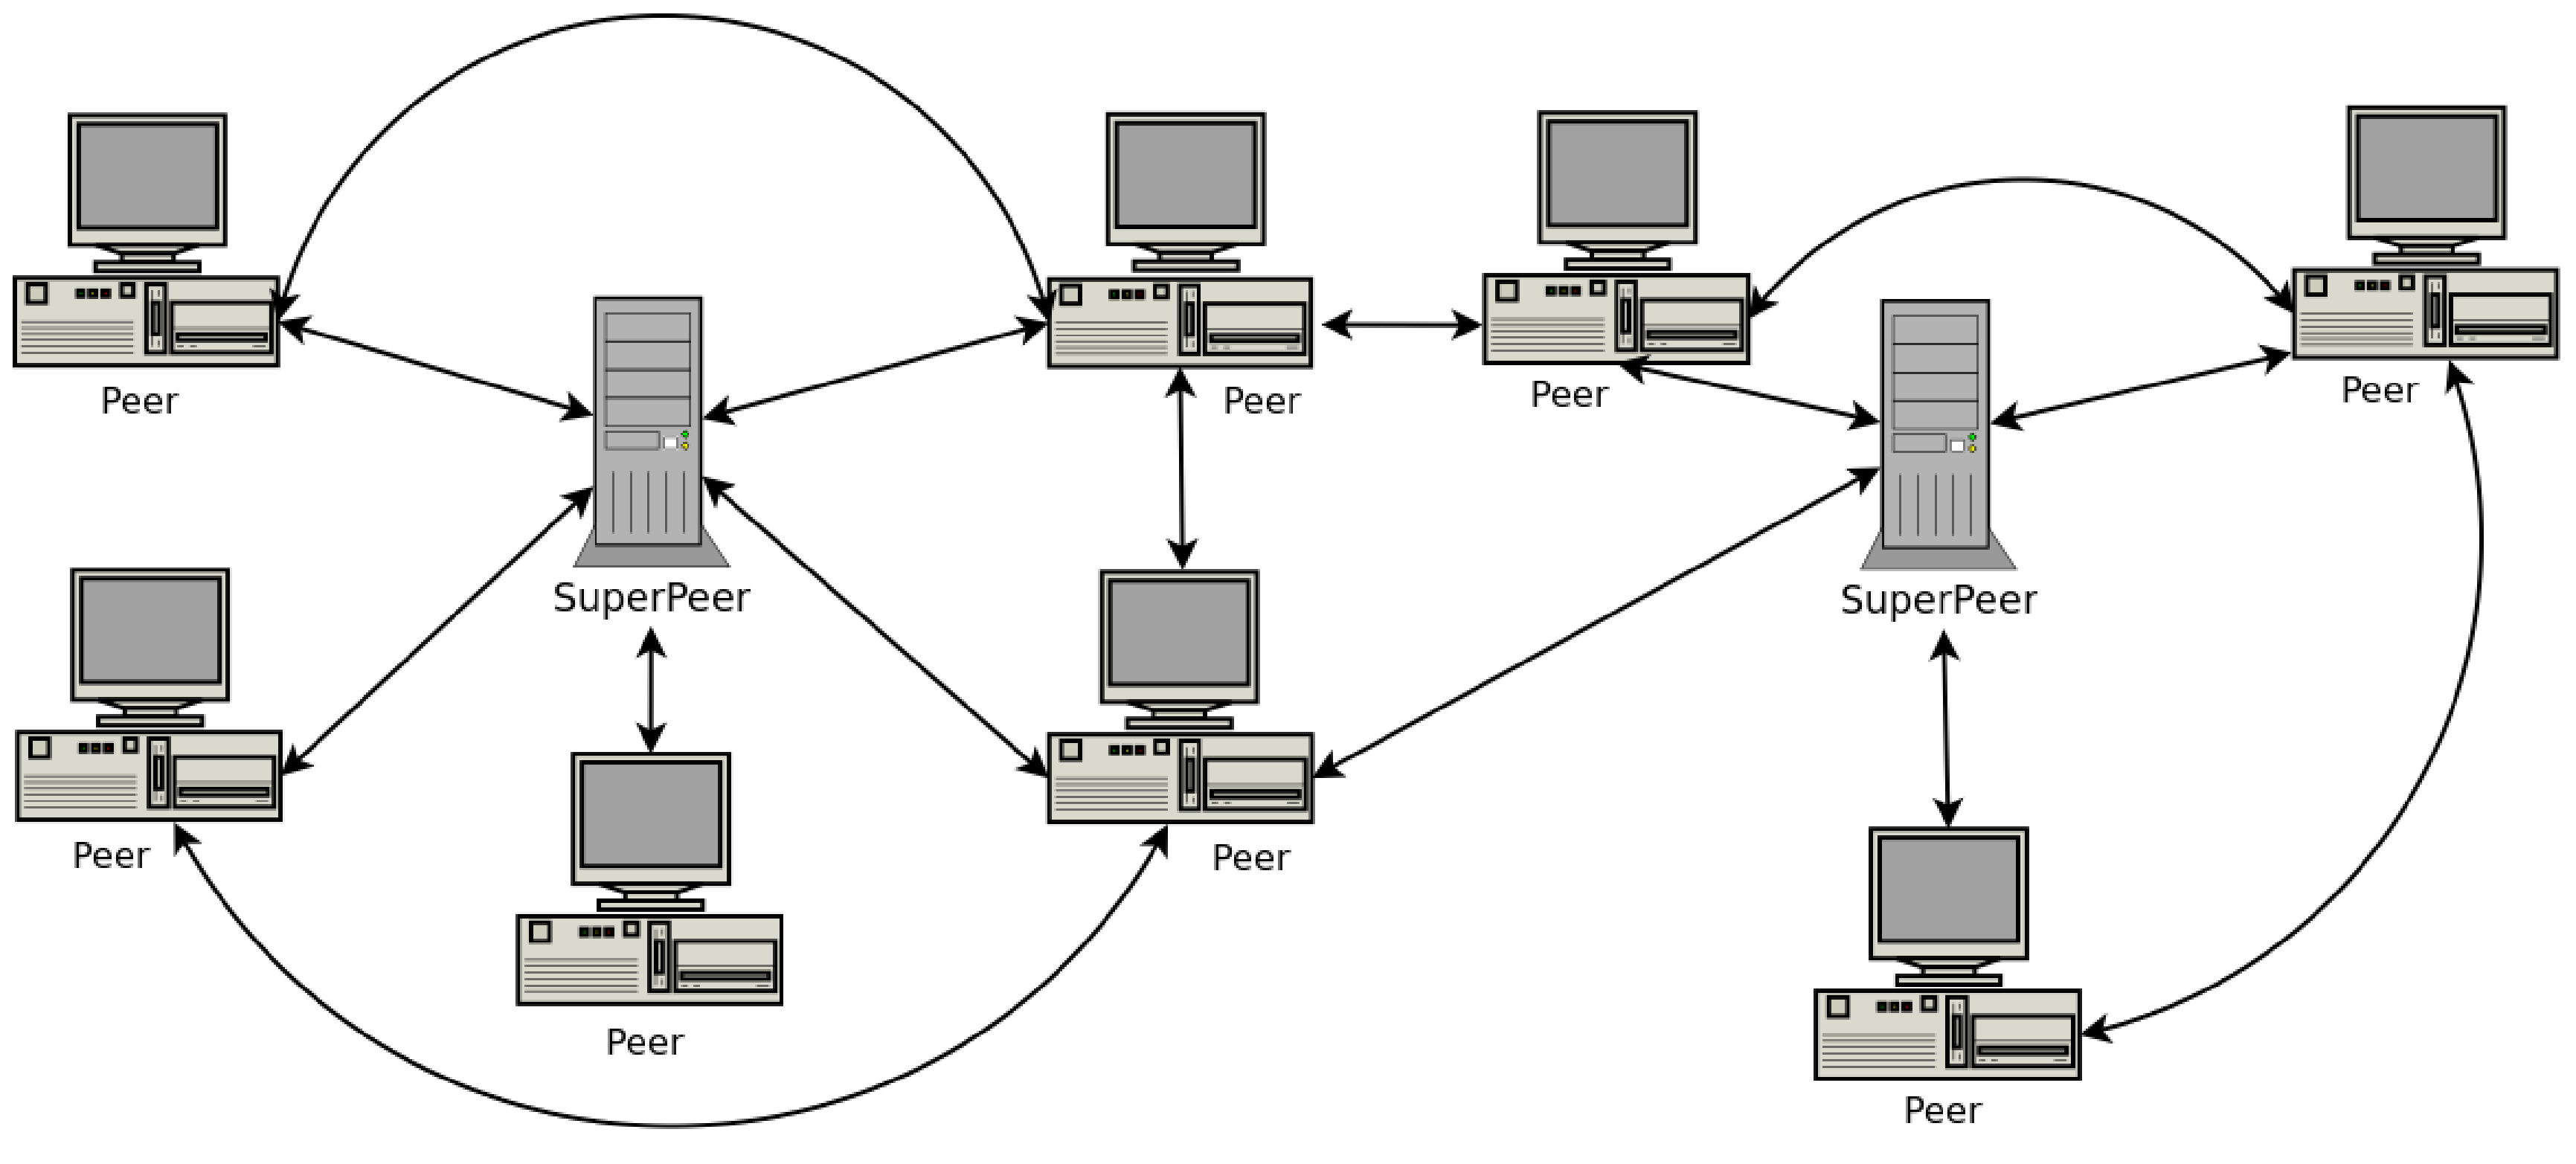
\includegraphics[width=0.7\textwidth]{hibrido}}\\
\subfigure{\includegraphics[width=0.4\textwidth]{decentralizado}}
\caption{From top to bottom. Centralised, hybrid and decentralised architectures.}
\label{fig:p2parchitectures}
\end{figure}
% De dónde lo has sacado? Cita la fuente, si lo has dibujado tú di
% ``inspirado en'' - JJ
% Lo he dibujao yo con dia. Inspirado en?, no se a que te refieres. - Juanlu



\clearpage
\subsection{Application areas}
\label{sec:p2papplication}
%%%%%%%%%%%%%%%%%%%%%%%%%%%%%%%%%%%%%%%%%%%%%%%%%%%%%%%%%%%%%%%%%%%%%%%%%%%%%%%


P2P systems have been widely used and mainly developed for file-sharing applications \cite{napstervsgnutella}. Nevertheless, the power for the harnessing of distributed resources -storage, computing power or human presence-  has attracted the attention of researchers from different areas into P2P systems. Thus, Mobile ad-hoc networks (MANET) can been modelled following a P2P approach \cite{manetp2p}, Voice over IP (VoIP) protocols can be understood as an instance of P2P protocols \cite{voipp2p} or idle cycles are used for computing applications \cite{deathtaxes}. In the widest sense, P2P is a key for understanding, approaching and modelling distributed resources providing a single coherent view of the system. The following points summarise four of the main application areas in which P2P systems are applied nowadays. 

\subsubsection{File-sharing}

    P2P systems were initially thought for this kind of applications. File-sharing P2P systems are platforms for the interchange of files between different final-users. Each one of these users is at the same time a service provider and a consumer requesting contents from other users. Therefore, contents had to be allocated in an addressable way in order of being retrieved by any user willing to obtain them. Depending on the system architecture, the \emph{look-up} problem can be addressed in a centralised way such in Napster \cite{napstervsgnutella}, in a decentralised way such in Gnutella 0.4 \cite{gnutella04} or in an hybrid way such in Gnutella 06 \cite{gnutella06}.

\subsubsection{VoIP and Instant Messaging}

    Voice has been recently incorporated to traditional instant messaging technology. Applications such MSN Messenger or Net2Phone use traditional VoIP protocols such as SIP or H.323 \cite{sip,h323}. Nevertheless, the most extended VoIP application nowadays is Skype, a P2P based VoIP protocol. Lisha and Junzhou show in \cite{voipp2p} that \emph{QoS} is rather similar between traditional and P2P approaches. However, the great advantage of using such P2P based approach is that it can solve NAT and firewall problems.


\subsubsection{Mobile ad-hoc networks (MANET)}

    MANETs are networks of sensors designed to collect information from the inside of a given phenomenon under study. The fields of application are numerous going from e.g. traffic jams control to glacial monitoring \cite{manetapplications}. The basic features of sensors include sensing the environment, processing the data and communicate with each other in a collaborative way. To this aim, networking techniques require of self-organised protocols in order to cope with an ad-hoc and changing environment in which the position and persistence of the sensors is unreliable. At this point, P2P techniques are helpful and are widely used in MANETs for the management of decentralised topologies, the probabilistic multi-casting of  information in multi-hop architectures, the resilience of the system to sensors failures and the scale-up of the network size \cite{manetp2p}.


\subsubsection{Cycle-sharing}

    Cycle-sharing P2P systems are distributed networks of heterogeneous single systems that contribute spare processor cycles for computing. A well-known example of application is the SETI@home project \cite{seti} searching for extraterrestrial intelligence patterns among a huge amount of radio signals collected from the spacial observatory of Arecibo in Puerto Rico. Despite strictly speaking SETI@home is based on Desktop Grid (DG) technology \cite{boinc}, the dividing line between both technologies is unclear and is mostly subject to differences in the network structure, centralised for DGs and decentralised for P2P. However, both technologies focus on the harnessing of computational power from a group of interconnected computers. Such source of computational power is  based in one or both of the following approaches:


%%%%%%%%%%%%%%%%%
\begin{itemize}
\item {\bf Volunteer Computing}:

    Volunteer Computing refers to distributed computing applications in which the source of computational power is aggregated from volunteers that willingly donate their idle CPU cycles to different research projects. In this case, cycle-sharing applications aim the harnessing of computing power at the edges of the Internet \cite{wehrle05:p2p}. 


\item {\bf Infrastructure applications}:

    There is no reason for limiting P2P technology to volunteer computing. As in the case of GRID technology, P2P systems can be hosted in private infrastructures. In fact, both technologies are compatible and they converge towards common places. Quoting Foster and Iamnitchi in \cite{deathtaxes} \emph{"$\dots$both are concerned with the same general problem, namely, the organisation of resource sharing within virtual communities$\dots$ $\dots$both take the same general approach$\dots$ $\dots$each has made genuine technical advances"}.
\end{itemize}
%%%%%%%%%%%%%%%%%

\subsubsection{Summary}

Among all the above mentioned application areas, this thesis might be catalogued as a study of viability on a cycle-sharing application. More concrete, an application based on distributed Evolutionary Algorithms. 
The main reason is that Evolutionary Algorithms performance depends on the complexity of the problems to be tackled. The more complex the problem instance, the larger the computing requirements. This fact leads to a sometimes prohibitively long time to solution that happens, for example, when tackling
many real-world problems. In order to reduce the execution time of EAs, this thesis presents a cycle-sharing P2P system as an alternative platform for the harnessing of computer power at a very low cost.

\clearpage
%%%%%%%%%%%%%%%%%%%%%%%%%%%%%%%%%%%%%%%%%%%%%%%%%%%%%%%%%%%%%%%%%%%%%%%%%%%%%%%
\section{Newscast Computing}
\label{sec:p2pnewscast}
%%%%%%%%%%%%%%%%%%%%%%%%%%%%%%%%%%%%%%%%%%%%%%%%%%%%%%%%%%%%%%%%%%%%%%%%%%%%%%%

% Todo esto tienes que haberlo definido antes. En todo caso, el
% protocolo no es dinámico, sino que es un protocolo para sistemas
% dinámicos. Habla siempre con propiedad. - JJ
% Modificado - Juanlu
As it has been mentioned at the introduction of this Chapter, we have chosen newscast to be the underlying P2P protocol in this thesis because it represents a good example of purely decentralised protocol that has shown to succeed in the main issues related to P2P computing such as massive scalability or fault tolerance. This section describes the design of its components and analyses the runtime dynamics of the protocol.

Newscast is a self-organised gossipping protocol for the maintenance of dynamic unstructured P2P
overlay networks \cite{jelasity:newscast}. Without any central services or servers, newscast differs from other similar approaches \cite{gnutella04,chord,can,pastry,tapestry} by its simplicity and scalability:

\begin{enumerate}
\item The membership management follows a extremely simple protocol: In
      order to join a group, a given node just has to contact any node
      within the system from which gets a list of its neighbours
      members. Additionally, to leave the group, the node just requires
      to stop communicating for a predefined time.

\item The dynamics of the system follow a probabilistic scheme able to keep a self-organised equilibrium at a macroscopic level. Such an equilibrium emerges from the loosely-coupled and decentralised run of the protocol within the different and independent nodes. The emerging macro-structure behaves as a small-world \cite{wattsstrogatz} allowing a scalable way for disseminating information and, therefore, making the system suitable for distributed computing.

\item Despite the simplicity of the scheme, newscast is fault-tolerant and exhibits a graceful degradation without requiring an extra mechanism other than its own emergent macro-behaviour \cite{spyros:robustscalable}.
\end{enumerate}



Algorithm \ref{alg:newscast} shows the pseudo-code of the newscast protocol. Each node 
keeps its own set of neighbours in a cache that contains $c \in \N$ entries, referring to $c$ other nodes in the network without duplicates. Each entry provides a reference to the node in which it was created and a time-stamp of the entry creation (allowing the replacement of old items).



%%%%%%%%%%%%%%%%%%%%%%
\begin{algorithm}
\caption{Newscast protocol in $node_i$}
\label{alg:newscast}
\scriptsize
\begin{algorithmic}


\STATE {\large Active Thread}
\LOOP 
\STATE wait $t_r$
\STATE $node_j$ $\Leftarrow$ Uniformly random selected node from $Cache_i$
\STATE send $Cache_i$ to $node_j$
\STATE receive $Cache_j$ from $node_j$
\STATE $Cache_i$ $\Leftarrow$ Aggregate ($Cache_i$,$Cache_j$)
\ENDLOOP
\STATE
\STATE {\large Passive Thread}
\LOOP
\STATE wait $Cache_k$ from $node_k$
\STATE send $Cache_i$ to $node_k$
\STATE $Cache_i$ $\Leftarrow$ Aggregate ($Cache_i$,$Cache_k$)
\ENDLOOP
\STATE
\STATE {\large $Cache_{aggregated}$ $\Leftarrow$ Aggregate($Cache_a$,$Cache_b$)}
\STATE $Cache_{aggregated} \Leftarrow Cache_a \cup Cache_b$
\STATE Keep the $c$ freshest items in $Cache_{aggregated}$ according with the time-stamp.
\end{algorithmic}
\end{algorithm}
%%%%%%%%%%%%%%%%%%%%%%


There are two different tasks that the algorithm carries out within each
node. The active thread which pro-actively initiates a cache exchange once every cycle (one cycle takes $t_r$ time units) and the passive
thread that waits for data-exchange requests. 

Every cycle each $node_i$ initiates a cache exchange.
It selects randomly a neighbour $node_j$ from its $Cache_i$ with uniform probability.
Then $node_i$ and $node_j$ exchange their caches and merge them following an aggregation function.
In this case, the aggregation consists of picking the freshest $c$ items from $Cache_i \cup Cache_j$ 
and merging them into a single cache that $node_i$ and $node_j$ will share.

\subsection{Communication Graph Series}
%%%%%%%%%%%%%%%%%%%%%%%%%%%%%%%%%%%%%%%%%%%%%%%%%%%%%%%%%%%%%%%%%%%%%%%%%%%%%%%

The dynamic sequence of relations between the different nodes defines a
series of communication {\em digraphs} (directed graphs) $D_t$ at time
$t$ starting, therefore, at $D_0$. In order to analyse the graph
subseries $D_{it_r} (i=0,\dots,N)$, we assume that a complete
communication cycle occurs within a time interval
$[it_r,(i+1)t_r]$. Given  the low communication exchange calls
frequencies (this property will be analysed in Section
\ref{sec:informationdissemination} around the results in
Fig. \ref{fig:informationexchange}) this assumption is not unrealistic
as long as the information exchange is short with respect to $t_r$.

In order to complete the characterisation of the graph series, we will analyse two of the most relevant properties in the communication graph $G_t$ obtained from dropping the orientation in $D_t$: the average path length and the clustering coefficient. The average path length of a node $n_i$ is the average of the minimal path between $n_i$ and the rest of nodes while the clustering coefficient of $n_i$ represents the fraction of its neighbours which are also neighbours between them. 



\subsection{Bootstrapping and Convergence}
\label{sec:bootstrapping}
%%%%%%%%%%%%%%%%%%%%%%%%%%%%%%%%%%%%%%%%%%%%%%%%%%%%%%%%%%%%%%%%%%%%%%%%%%%%%%%

% Esto quién lo ha hecho? Forma parte de la tesis? Lo has hecho tú? Deja
% claro si es una aportación o no - JJ
% He añadido: "It reproduces the results of the newscast seminal paper in []" - Juanlu
This section studies the self-organised dynamics of the newscast
communication graph series showing that independently of the
initialisation criterion, the graph is able to bootstrap and converge to
stable conditions. It reproduces the results of the newscast seminal paper in  \cite{jelasity:newscast}.  Figure \ref{fig:fromrandomws} represents the
convergence of the graph series bootstrapping from a random and a
small-world graph at $G_0$. In quite an early stage, i.e. around
$G_{12t_r}$, the graph converges to an state of dynamic
equilibrium with independence of the initial graph $G_0$. 

\begin{figure*}[htbp]
\centering
\subfigure{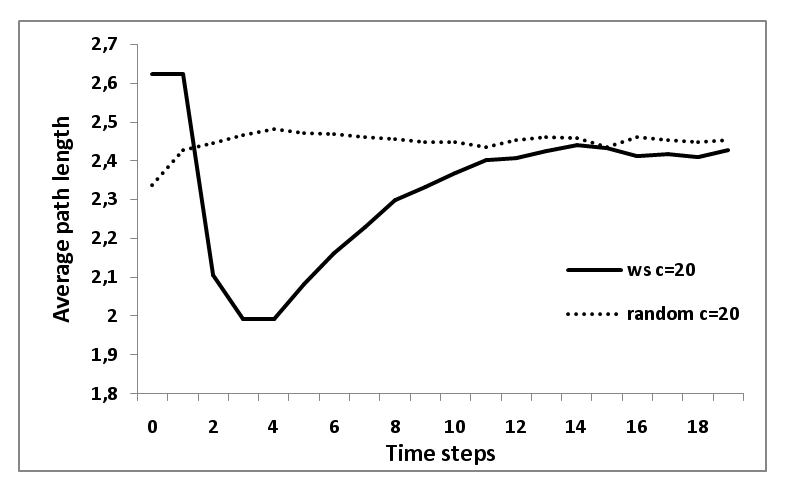
\includegraphics[width=0.7\textwidth]{lengthrandomws}}\\
\subfigure{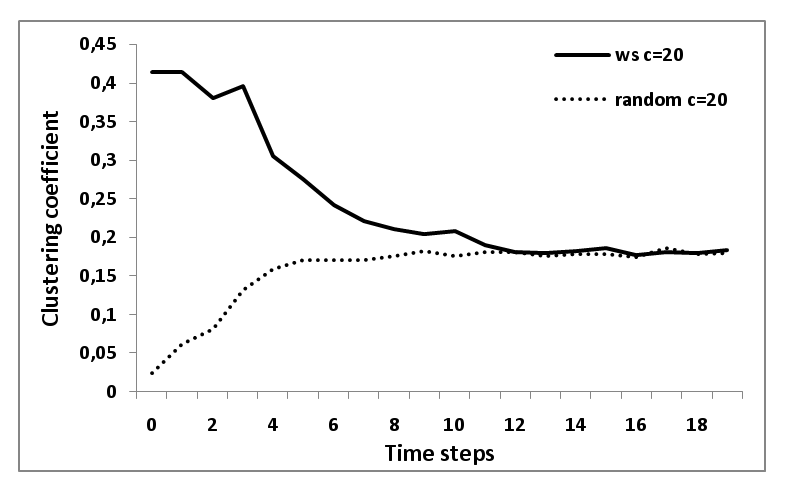
\includegraphics[width=0.7\textwidth]{clusteringrandomws}}
\caption{Convergence of the average path length ({\em up}) and
 clustering coefficient ({\em down}) bootstrapping from a random and a
 Watts-Strogatz (ws) graph for a number of nodes $n=1600$. The graph can be seen to converge to the same values within the interval
 $G_{0t_r-20t_r}$ showing the independence of the protocol convergence
% De _todo_ el protocolo? Dí qué parte o efecto o atributo es independiente - JJ
% Cierto, es independiente con respecto a la convergencia del protocolo - Juanlu
with respect to the initialisation criterion.}
\label{fig:fromrandomws}
\end{figure*}

Nevertheless, the cache size ($c$) plays here an important role. It represents the maximum degree of a node, and therefore, influences the average path length and the clustering coefficient. For example, Figure \ref{fig:fromrandom} shows newscast converging to different values depending on $c$.

\begin{figure*}[htbp]
\centering
\subfigure{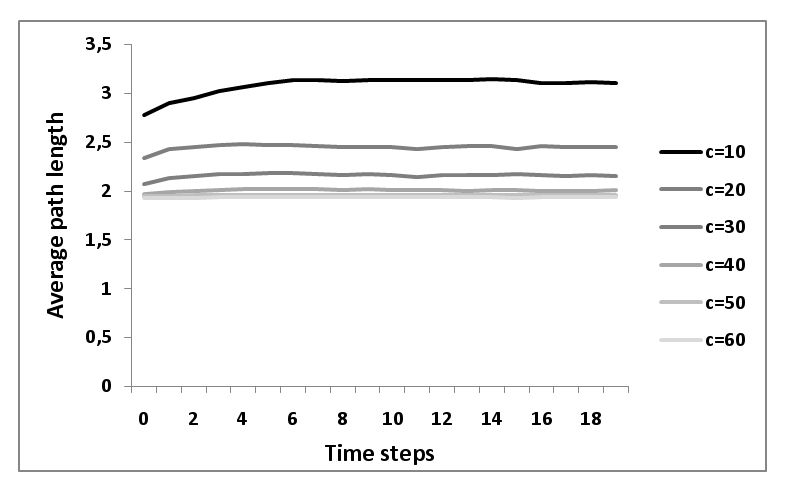
\includegraphics[width=0.7\textwidth]{lengthfromrandom}}\\
\subfigure{\includegraphics[width=0.7\textwidth]{clusteringfromrandom}}
\caption{Convergence of the average path length ({\em up}) and clustering coefficient ({\em down}) bootstrapping from a random graph for different cache sizes and a number of nodes $n=1600$}
\label{fig:fromrandom}
\end{figure*}


In addition, Figure \ref{fig:newscast} depicts the influence of the cache size on the average path length and the clustering coefficient for different network sizes. A smaller $c$ implies a higher clustering coefficient and also a higher average path length.

\begin{figure*}[htbp]
\centering
\subfigure{\includegraphics[width=0.7\textwidth]{length}}\\
\subfigure{\includegraphics[width=0.7\textwidth]{clustering}}
\caption{Converged average path length ({\em up}) and clustering coefficient ({\em down}) for $G_{40t_r}$ and different network and cache sizes ($c$).}
\label{fig:newscast}
\end{figure*}

Based on such features, a newscast graph can behave as a small-world by tuning $c$ to the adequate values. In this sense, Jelasity and van Steen state in \cite{jelasity:newscast} that the intended normal setting of newscast is $c \ll n$; for $c \ll n$, newscast has the small average path length of random graphs but, as shown in Figure \ref{fig:randomnws}, a much higher clustering coefficient \cite{spyros:robustscalable}.


\begin{figure*}[htbp]
\centering
\subfigure{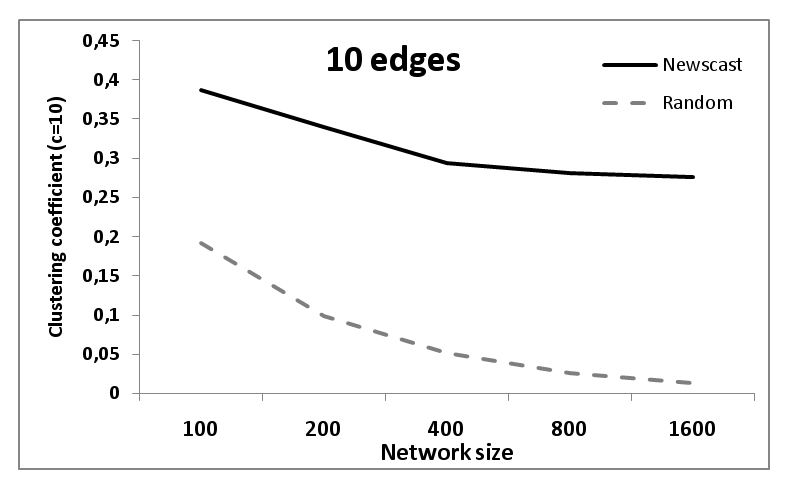
\includegraphics[width=0.7\textwidth]{randomnwsc10}}\\
\subfigure{\includegraphics[width=0.7\textwidth]{randomnwsc20}}
\caption{Clustering coefficients for equivalent random and newscast graphs (i.e. nodes have the same number of edges, ten on the upper figure and twenty at the bottom one). The higher values in the newscast graphs point to a small-world topology.}
\label{fig:randomnws}
\end{figure*}

\subsection{Robustness}
\label{sec:newscastrobustness}
%%%%%%%%%%%%%%%%%%%%%%%%%%%%%%%%%%%%%%%%%%%%%%%%%%%%%%%%%%%%%%%%%%%%%%%%%%%%%%%

One of the important issues regarding P2P computing is the robustness of the underlying protocols such as newscast, that is, protocols describe the dynamics of the communication graph series ($G_t$) in a continuous changing environment. In this section, we consider two important aspects regarding the robustness of the newscast protocol\footnote{Results are reproduced from \cite{spyros:robustscalable}.}.

\begin{enumerate}
\item The probability of spontaneous partitioning of $G_t$.
\item The robustness of newscast to node removals.
\end{enumerate}


%%%%%%%%%%%%%%%%% 
\begin{figure}[htbp]
\centerline{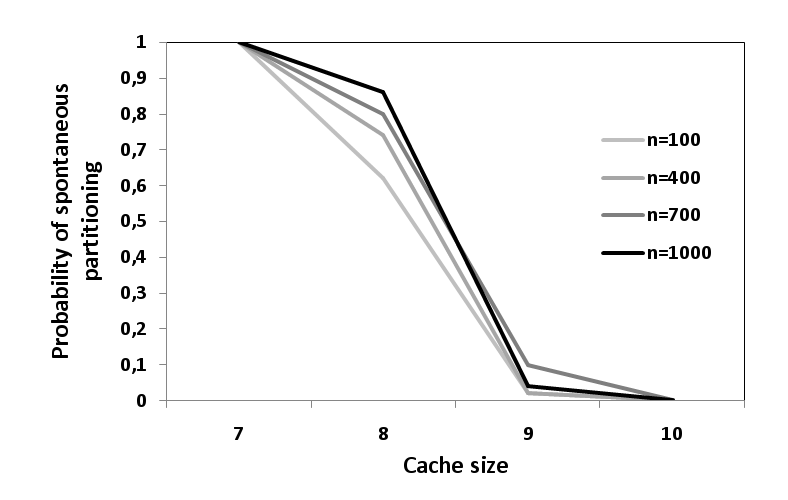
\includegraphics[width=0.8\textwidth]{spontaneous}}
\caption{Probability of spontaneous graph partitioning as a function of the cache size. Probabilities are obtained from 50 independent runs starting at the random graph $G_0$ until $G_{20000t_r}$ or partitioning.}
\label{fig:spontaneous}
\end{figure}
%%%%%%%%%%%%%%%%% 

The spontaneous partitioning of the communication graph series means that a subgraph becomes disconnected within the interval $G_{0-t}$ as a consequence of the protocol dynamics. Figure \ref{fig:spontaneous} shows that in newscast the probability of spontaneous partitioning is mainly influenced by the cache size $c$. Despite the results showing that the null probability is reached for $c=10$, it has to be considered that results are obtained over 50 independent runs for relatively small networks within the interval $G_{0-20000t_r}$ and, therefore, it might be still possible to get a partition considering larger networks, a larger number of runs or a larger time interval. In this sense, the seminal study in \cite{jelasity:newscast} extends such results and establishes that the probability of spontaneous partitioning is almost negligible from $c=20$ ahead.


%%%%%%%%%%%%%%%%% 
\begin{figure*}[htbp]
\centering
\subfigure{\includegraphics[width=0.7\textwidth]{numberclusters}}\\
\subfigure{\includegraphics[width=0.7\textwidth]{sizeofcluster}}
\caption{Partitioning of the communication graph as a function of the percentage of removed nodes in $G_0$ (random graph) and the newscast subgraph $G_{20t_r}$. Results are averaged from 50 independent runs and n=5000.}
\label{fig:numberclusters}
\end{figure*}
%%%%%%%%%%%%%%%%% 

Nevertheless, previous results on the spontaneous partitioning of $G_t$ do not take into account peers failures which is an inherent feature of Peer-to-Peer systems known as \emph{churn} \cite{Stutzbach06Understanding}. Churn emerges from the collective dynamics of peers joining and leaving the system. Given that the running platforms use to be highly dynamic (e.g. the Internet) protocols have to be well-suited for tolerating faults. Therefore, we study in Figure \ref{fig:numberclusters} the robustness of newscast in an scenario in which nodes are removed up to none is left. It can be seen how newscast inherits the robust behaviour of random graphs, especially when $c$ is large. On the one hand, the graph remains connected until a large percentage of nodes are removed, e.g. for $c=40$, $90\%$ of the nodes have to be removed to get a partition of the graph. On the other hand, most of the nodes remain in the larger cluster once the partition takes place. 



\subsection{Dissemination of the information}
\label{sec:informationdissemination}
%%%%%%%%%%%%%%%%%%%%%%%%%%%%%%%%%%%%%%%%%%%%%%%%%%%%%%%%%%%%%%%%%%%%%%%%%%%%%%%

In order to make distributed computing possible, a key element in a distributed system is having a reliable information flow. Taking into account the decentralised and unreliable nature of P2P systems, newscast guarantees a scalable and reliable dissemination of the information by implementing a probabilistic \emph{epidemic} multi-casting scheme. As in infectious diseases, a piece of information is able to "infect" the "healthy" neighbourhood of a given carrier node. The speed of dissemination is high at the small-world structure of the communication graph and the process is likely to "infect" the whole graph in few time steps.

Such an effect can be visualised in the following experiment. At time $0$ one node produces a piece of information (so-called a news item) that is sent to one of the neighbours every time-step. Once that a node is "infected" begins to act as a replicant and sends the news item to its neighbourhood. This way, Figure \ref{fig:takeover} shows the proportion of "infected" nodes as a function of time. To this end, a complete graph and two different parameterised newscast graph were considered. 

%%%%%%%%%%%%%%%%%  
\begin{figure*}[htbp]
\centerline{\includegraphics[width=0.8\textwidth]{disseminationnewscast}
}
\caption{Dissemination speed of a news item through the entire network for a complete graph and two newscast graphs with $c=10$ and $c=20$. Results are averaged from 50 independent runs for a network size of $n=1600$.}
\label{fig:takeover}
\end{figure*}
%%%%%%%%%%%%%%%%% 

Similar curves in Figure \ref{fig:takeover} denote equivalent speeds in the dissemination of information induced by both kind of topologies.  Nevertheless, the node degree in complete graphs of size $n$ is $n-1$ while the average degree in newscast is approximately $2c$ pointing out a better scalability of the small-world approach given that the intended normal setting of newscast is $c \ll n$.



%%%%%%%%%%%%%%%%% 
\begin{figure}[htbp]
\centerline{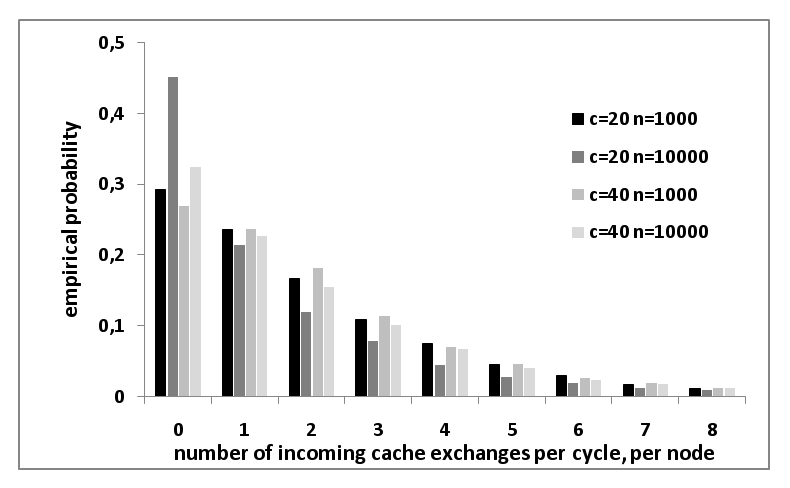
\includegraphics[width=0.8\textwidth]{informationexchange}}
\caption{ Information exchange calls probability in a fixed node during a time interval $t_r$ (cycle). Results are estimated in the graph series $D_0 \dots D_{10000t_r}$ where $D_0$ is a random graph.}
\label{fig:informationexchange}
\end{figure}
%%%%%%%%%%%%%%%%% 

\bigskip
\bigskip

In addition to a lower node degree than in complete graphs, the low frequencies of the information exchange calls are a good indicator of the scalability of the protocol as depicted in Figure \ref{fig:informationexchange}. Independently of the network and cache sizes (i.e. assuming $c \ll n$), a node receives at any given cycle $t_r$ less than 4 information requests with probability $p > 0.8$ and less than 8 with $p > 0.98$. Therefore, a randomly chosen node is likely to process few requests in a cycle. Whenever $t_r$ is large enough with respect to a single request (e.g. 20 times larger) the protocol run does not represent a bottleneck on the system even when considering large network sizes.



%%%%%%%%%%%%%%%%%%%%%%%%%%%%%%%%%%%%%%%%%%%%%%%%%%%%%%%%%%%%%%%%%%%%%%%%%%%%%%%
\section{Summary}
\label{sec:p2pconclusions}
%%%%%%%%%%%%%%%%%%%%%%%%%%%%%%%%%%%%%%%%%%%%%%%%%%%%%%%%%%%%%%%%%%%%%%%%%%%%%%%

This chapter provides a general overview of the Peer-to-Peer Computing area. In order to provide an adequate understanding of P2P systems and a general taxonomy of the application areas, the system architectures and the different ways of approaching fully-decentralised schemes is introduced. 

In addition, the chapter focuses on an exhaustive analysis of the newscast protocol that will be used within this thesis as the underlying running platform for the experiments.
Newscast is a decentralised gossip-based protocol that follows an \emph{epidemic} scheme for disseminating the information. Despite its simplicity, it is a robust and scalable protocol able to self-organise the relations between peers into a small-world communication graph. That is, independently of the initial conditions, the system converges to an state of dynamic equilibrium that behaves asymptotically as an small-world graph.



%%%%%%%%%%%%%% Bibliografia %%%%%%%%%%%%%%%

%\bibliographystyle{alpha}  % Eliminarlo al compilar el documento maestro, ponerlo para compilarlo separado
%\bibliography{p2pcomputing}%,gprop,mmitchell,zmich,hilera,fjmm,ripley,rbeale,jhertz,mag}       % Eliminarlo al compilar el documento maestro, ponerlo para compilarlo separado

%\end{document}             % Eliminarlo al compilar el documento maestro, ponerlo para compilarlo separado